% !TEX root = mainthesis.tex
%Chapter 6


\newcommand{\reffig}[1]{Fig.~\ref{#1}}
\newcommand{\refeq}[1]{Eq.~(\ref{#1})}

\renewcommand{\thechapter}{6}

\chapter{Synthetic clock states}
\label{ch:clock_states}

 Most of our previous experiments used the hyperfine $\ket{m_F}$ states as effective spins and dressed them with an RF or Raman laser field. However, due to the linear dependence of their energies with respect to magnetic field, and the fact that we had two other AMO labs generating large magnetic fields and an elevator nearby, we always had to take special care to stabilize the magnetic field on the lab (see~\ref{sec:ptai} for details on magnetic field stabilization using partial transfer absorption imaging). Our system is not the only one suffering from this issues; decoherence of quantum systems due to uncontrolled fluctuations of the environment presents fundamental obstacles in quantum science. One way to go around this is to use of first order insensitive `clock' transitions which are insensitive to such fluctuations, however, they are not present in all systems or for arbitrary system parameters. Remarkably, under almost all circumstances, clock transitions can be synthesized using dynamical decoupling protocols. These protocols involve driving the system with an external oscillatory field, resulting in a dynamically protected `dressed' system.

The idea of using continuous dynamical decoupling (CDD) in the lab came from a theoretical proposal to engineer Rashba type SOC using Raman beams and a strong RF field~\cite{campbell_rashba_2016}. We decided to implement CDD to create `synthetic clock states', which was one of the ingredients in this proposal, as an intermediate step towards our final goal of engineering Rashba SOC. Just like with Fourier spectroscopy, CDD became a workhorse of the lab both for the stability it provides against environmental fluctuations but also because it has given us access to non-zero matrix coupling elements that we otherwise would not have when working with the bare $\ket{m_F}$ states. We have continued to use CDD  not only for engineering Rashba SOC (Chapter~\ref{ch:Rashba}) but also to engineer subwavelength optical lattices (Chapter~\ref{ch:raman_lattice}) and Hofstadter cylinders (\note{maybe not a Chapter since there are already too many...}). 

This Chapter discusses the implementation of continuous dynamical decoupling (CCD) in our system of ultra-cold atoms. First I will give a general overview of dynamical decoupling and continuous dynamical decoupling techniques. Then I will describe our implementation of CDD using a strong RF field that couples the $F=1$ hyperfine manifold of $\Rb87$. Finally I discuss an implementation of concatenated CDD that renders the system first-order insensitive to both magnetic field noise and noise in the control field. This work was published in~\cite{trypogeorgos_synthetic_2018} and was done in parallel with~\cite{anderson_continuously_2018}.

\section{Basic principles of CDD}

The use of dynamical decoupling protocols as a way of beating decoherence was first theoretically proposed in~\cite{viola_dynamical_1998}.

A number of dynamical decoupling protocols, pulsed or continuous, have been shown to isolate quantum systems from low-frequency environmental noise~\cite{cohen_continuous_2017,fanchini_continuously_2007,aharon_fully_2016,biercuk_optimized_2009,cai_robust_2012,bermudez_robust_2012,baumgart_ultrasensitive_2016,kazakov_magic_2015,sarkany_controlling_2014}. Continuous dynamical decoupling (CDD) relies on the application of time-periodic continuous control fields, rather than a series of quantum-logic pulses. Unlike conventional dynamical decoupling, CDD does not require any encoding overhead or quantum feedback measurements. 

Thus far, CDD has inoculated multi-level systems in nitrogen vacancy centers in diamond, nuclear magnetic resonance experiments, and trapped atomic ions~\cite{laucht_dressed_2017,farfurnik_experimental_2017,noguchi_generation_2012,golter_protecting_2014,timoney_quantum_2011,webster_simple_2013,barfuss_strong_2015,rohr_synchronizing_2014}, from spatiotemporal magnetic field fluctuations.We demonstrate CDD in atomic BECs producing a protected three-level system of dressed-states, whose Hamiltonian is fully controllable. The CDD-protected states are sensitive to fluctuations of the amplitude of the control field, and we  demonstrate that a second coupling field protects against those in a concatenated manner~\cite{cohen_continuous_2017,farfurnik_experimental_2017,cai_robust_2012}.
Some Bloch spheres and an explanation


\section{CDD of a spin-1 system}
\begin{figure}[!!h]
    \centering
    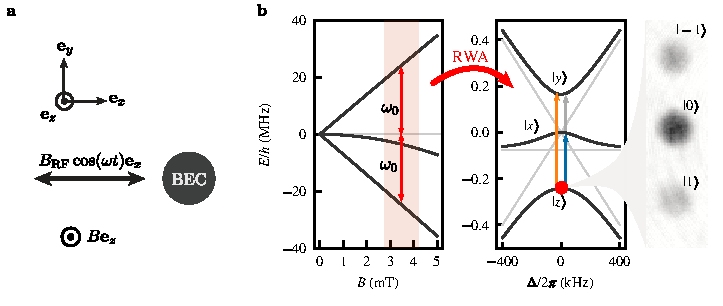
\includegraphics[]{Figures/Chapter6/fig1a.pdf}
    \caption[Implementing CCD.]{{\bf a.} Setup for implementing CCD using a strong RF magnetic field. {\bf b.}  Left: dependence of the $5^2S_{1/2}$, $F=1$ ground state of $\Rb87$ on magnetic field, where the quadratic dependence of the $\ket{m_F=0}$ state's Zeeman shift has been exaggerated so it is visible on the same scale.
    Center: energies of the $\xyz$ eigenstates, for $\Omega/2\pi=\SI{200}{kHz}$ (black curves) and $\Omega=0$ (grey curves).
    Right: TOF absorption image of $\ket{z}$ at $\Delta=0$, showing the constituent $m_F$ states.
    }
    \label{fig:1}
\end{figure}

We implemented CDD using a strong radio-frequency (RF) magnetic field with strength $\Omega$, that linked the three $m_F$ states comprising the $F=1$ electronic ground state manifold of $\Rb87$.
The RF field was linearly polarized along ${\bf e}_x$, and had angular frequency $\omega$ close to the Larmor frequency $\omega_0 = g_F \mu_{\rm B} B_0$ from a magnetic field $B_0 {\bf e}_z$; $g_F$ is the Lande $g$-factor and $\mu_{\rm B}$ is the Bohr magneton. Our system was described by the RF Hamiltonian described in~\ref{seq:rf_coupling}

\begin{equation}
    \hat{H} = \hbar\Delta\fz+\hbar\epsilon(\fz^2-\hat{\mathbb{1}})+ \hbar\Omega \fx,
    \label{eq:h0}
\end{equation}
with detuning $\Delta=\omega-\omega_0$; quadratic Zeeman shift $\epsilon$; spin-1 angular momentum operators $\hat F_{x,y,z}$; and identity operator $\hat{\mathbb 1}$.  

\subsection{The $\xyz$ states}

The eigenstates of Equation~\ref{eq:h0} are linear combinations of $\ket{m_F=0,\pm1}$. We denote this states by $\ket{x}$, $\ket{y}$ and $\ket{z}$. The eigenvalues are the root of the characteristic cubic polynomial $H(\lambda)=\Delta^2\epsilon + (\Delta^2 + \Omega^2) \lambda - \epsilon \lambda^2 - \lambda^3$ and are even functions with respect to $\Delta$ as can be seen by the leading order expansion for $\Delta\to 0$
\begin{align}
    \omega_x =& -\frac{\epsilon}{\Omega^2} \Delta^2 + \mathcal{O}(\Delta^4), \nonumber \\
    \omega_y =& \frac 12 (-\epsilon + \tilde\Omega) - \frac{(\epsilon + \tilde\Omega)}{-\epsilon^2-4\Omega^2+\epsilon\tilde\Omega} \Delta^2 + \mathcal{O}(\Delta^4), \label{eq:exp} \\
    \omega_z =& \frac 12 (-\epsilon - \tilde\Omega) + \frac{(\epsilon - \tilde\Omega)}{\epsilon^2+4\Omega^2+\epsilon\tilde\Omega} \Delta^2 + \mathcal{O}(\Delta^4), \nonumber
\end{align}
where $\tilde\Omega=\sqrt{\Omega^2+\epsilon^2}$
The energy differences $\hbar\omega_{xy}$, $\hbar\omega_{zy}$ and $\hbar\omega_{zx}$ are only quadratically sensitive to $\Delta$ for $\Delta\ll\Omega$~\footnote{The energies are quadratic in $\Delta$ for $\Delta\ll\Omega$, and linear for $\Delta\gg\Omega$ with a slope of \SI{7}{MHz/mT}.} so that detuning fluctuations $\delta \Delta$ are suppressed to first order, making these a trio of synthetic clock states.


We focused on the $zx$ transition since the curvature of $\omega_x$ and $\omega_z$ has the same sign for $\epsilon < \tilde \Omega$ (\refeq{eq:exp}).
Since the quadratic term changes curvature it can be made arbitrarily small.
However, this cancellation does not take place when we consider the dependence of $\epsilon$ on $\Delta$ from the Breit-Rabi expression.





The energy differences $\hbar\omega_{xy}$, $\hbar\omega_{zy}$ and $\hbar\omega_{zx}$ are only quadratically sensitive to $\Delta$ for $\Delta\ll\Omega$~\footnote{The energies are quadratic in $\Delta$ for $\Delta\ll\Omega$, and linear for $\Delta\gg\Omega$ with a slope of \SI{7}{MHz/mT}.} so that detuning fluctuations $\delta \Delta$ are suppressed to first order, making these a trio of synthetic clock states.

At an optimal $\Omega$, $\omega_{zx}$ depends quartically on $\Delta$~\cite{xu_coherence-protected_2012,rabl_strong_2009}. For $\Delta \gg \Omega$ the $\xyz$ states adiabatically connect to the corresponding $\ket{m_F=1,0,-1}$, states (\reffig{fig:1}b).
As $\Omega\rightarrow 0^+$ and for $\Delta=0$, the $\xyz$ states continuously approach the $\XYZ$ states familiar from quantum chemistry~\cite{cooper_reaching_2013}.
In contrast, as $\Omega\to\infty$ they become eigenstates of the $\hat F_x$ operator: $\ket{y,x,z} \to \ket{m_x=+1,0,-1}$.
Unlike for the $m_F$ basis, an oscillatory magnetic field can drive transitions between all pairs of the $\xyz$ states with non-zero transition matrix elements (see Appendix~\ref{app:xyz} for more details).



\textit{The $\xyz$ dressed basis}
\label{app:xyz}

The corresponding (non-normalized) eigenvectors are linear combinations of the $m_F$ basis states:
\begin{align}
    \ket x =& \ket{-1} + \ket{1}, \nonumber \\
    \ket y =& \ket{-1} -\frac{\epsilon + \tilde\Omega}{\sqrt 2 \Omega} \ket 0 + \ket 1, \\
    \ket z =& \ket{-1} -\frac{\epsilon - \tilde\Omega}{\sqrt 2 \Omega} \ket 0 + \ket 1. \nonumber
\end{align}

We measured the above decomposition of the $\xyz$ states to $m_F$ states using a projective measurement by abruptly turning off the dressing field $\Omega$ (see \reffig{fig:s1}).
\begin{figure*}[ht]
    \centering
    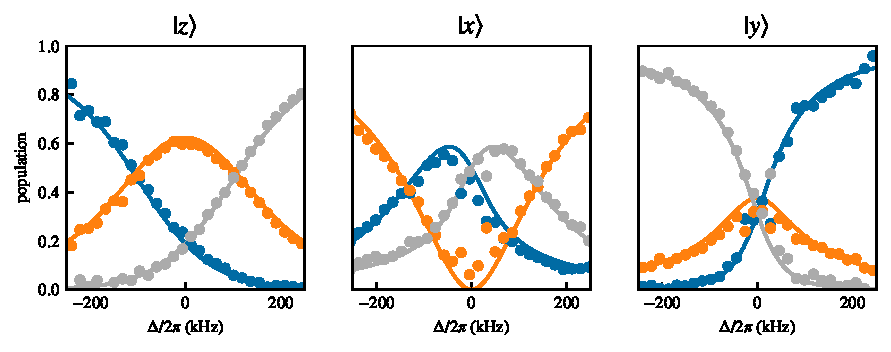
\includegraphics[]{Figures/Chapter6/figS11}
    \caption[State decomposition of the $\xyz$ states]{Decomposition of the $\xyz$ states on the $m_F$ basis for $\Omega/2\pi=\SI{145(1)}{kHz}$
    The $\ket{m_F=-1,0,1}$ states correspond to blue, orange, gray respectively.}
    \label{fig:s1}
\end{figure*}
\begin{figure*}[ht]
    \centering
    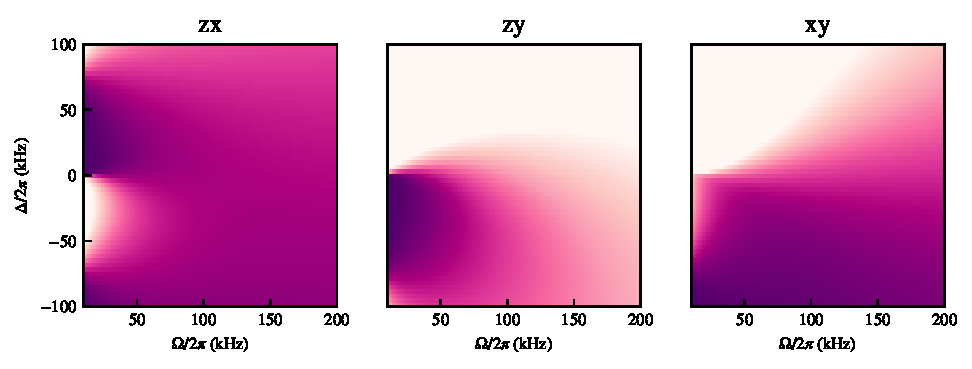
\includegraphics[]{Figures/Chapter6/figS12}
    \caption[Transition matrix elements over $\Omega$ and $\Delta$.]{Transition matrix elements over $\Omega$ and $\Delta$.
    There is an assymetry between coupling on the blue and red side of the resonance that corresponds to the counter- and co-rotating terms $\hat F_-$ and $\hat F_+$.}
    \label{fig:s12}
\end{figure*}


For $\Delta=0$ and small coupling $\Omega / \epsilon \to 0$ with regard to the quadratic shift the $\ket y$ and $\ket x$ become symmetric and antisymmetric superpositions of the $\ket{m_F=-1, 1}$ states while $\ket z$ is predominantly composed of $\ket 0$
\begin{align}
    \ket x &= \ket{1} - \ket{-1}, \nonumber \\
    \ket y &= \ket{1} + \ket{-1} + \frac{\Omega}{\epsilon}\ket 0, \\
    \ket z &= \frac{\Omega}{\epsilon}(\ket{1} + \ket{-1}) -\ket 0. \nonumber
\end{align}
On the other hand, when $\Omega\to\infty$ they are independent of the driving field amplitude and continuously approach the eigenstates of the $\hat F_x$ operator
\begin{align}
    \ket x &= \ket{1} - \ket{-1}, \nonumber \\
    \ket y &= \ket{1} + \sqrt 2 \ket 0 + \ket{-1}, \\
    \ket y &= \ket{1} - \sqrt 2 \ket 0 + \ket{-1}. \nonumber
\end{align}
The states adiabatically map to the $\ket{m_F}$ states for $\Delta \gg \Omega$ as shown in \reffig{fig:s1}.
For $\Delta/2\pi > \SI{200}{kHz}$ the $\xyz$ states are not yet fully deloaded to a single $m_F$ state since the population in other $m_F$ states is not negligible.
$\ket z$ maps to $\ket 1$ ($\ket{-1}$) for positive (negative) detuning; $\ket y$ maps in the exact opposite way to $\ket z$; and $\ket x$ always maps to $\ket 0$.
For large enough $\Delta$ the $zx$ and $xy$ transitions become degenerate and the system resembles an $F=1$ ground state at low magnetic field.
\begin{figure*}[ht]
    \centering
    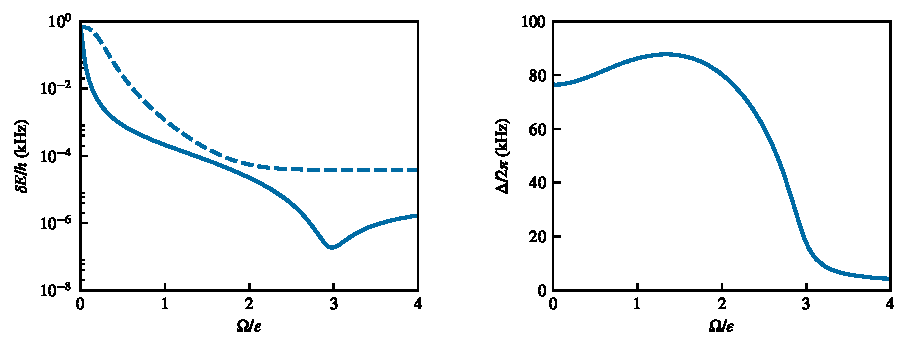
\includegraphics[]{Figures/Chapter6/figS13}
    \caption{Left: The optimum response (solid) of the $zx$ transition to detuning fluctuations allowing for finite $\Delta$ compared to $\Delta=0$ (dashed).
    Right: The values of $\Delta$ that correspond to the minimum derivative of $\omega_{zx}$.}
    \label{fig:sopt}
\end{figure*}
\begin{figure*}[ht]
    \centering
    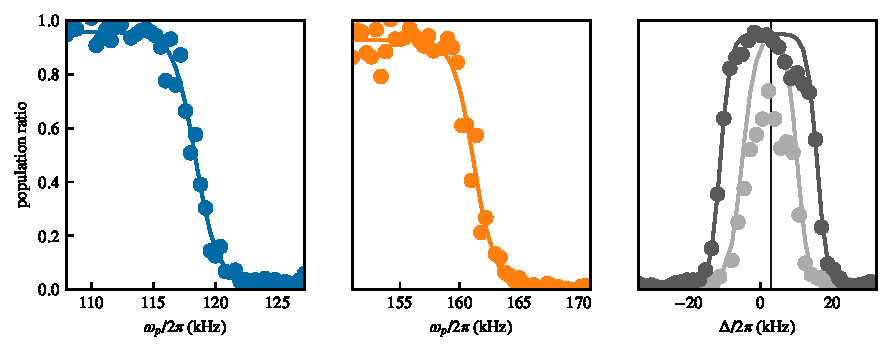
\includegraphics[]{Figures/Chapter6/figS2}
    \caption[]{Characteristic spectroscopy curves for the $zx$ (left) and $zy$ (middle) transitions.
    Two symmetric ARPs (right) define the resonant value of the magnetic field.
    The width of the peak gets smaller as $\Delta$ gets closer to the resonant value.
    Here $\Delta/2\pi=\SI{3}{kHz}$.}
    \label{fig:s2}
\end{figure*}







\textit{Transition matrix elements}
\label{app:me}
The $\XYZ$ states transform under the application of the spin-1 operators as $\epsilon_{jkl}\hat F_j \ket k= i\hbar \ket l$, so that a resonant probe field can induce transitions between at least one pair of states, irrespectively of its polarization.


The transition matrix elements between the $\xyz$ show a dependence on both $\Omega$ and $\Delta$ (see \reffig{fig:s12}).
For $\Omega \ll \epsilon$ the matrix elements correspond to those of the $\ket{m_F}$ basis and $\langle x \vert \hat F_+ \vert y \rangle = 0$ as expected by angular momentum selection rules.
When $\Omega$ and $\epsilon$ are comparable in magnitude al transition matrix elements are nonzero and the states can be coupled cyclically.
As $\Omega \gg \epsilon$ the $\ket z$ and $\ket y$ states decouple and the system resembles an `undressed basis' following similar selection rules.






\section{Experiment}

We coupled the dressed states using a weaker probe field with strength $\Omega_p$, polarized along ${\bf e}_y$ with angular frequency $\omega+\omega_p$ (\reffig{fig:1}a).
Using the rotating wave approximation (RWA) for the frame rotating at $\omega$ (valid when $\omega_0 \gg \Omega,\,\Omega_p,\,\omega_p$), the system is described by
\begin{equation}
    \hat{H} = \hbar\Delta\fz+\hbar\epsilon(\fz^2-\hat{\mathbb{1}})+ \hbar\Omega \fx
    + \hbar\Omega_p \left(\sin(\omega_p t) \fx + \cos(\omega_p t) \fy\right),
    \label{eq:h}
\end{equation}


\begin{figure}[!!h]
    \centering
    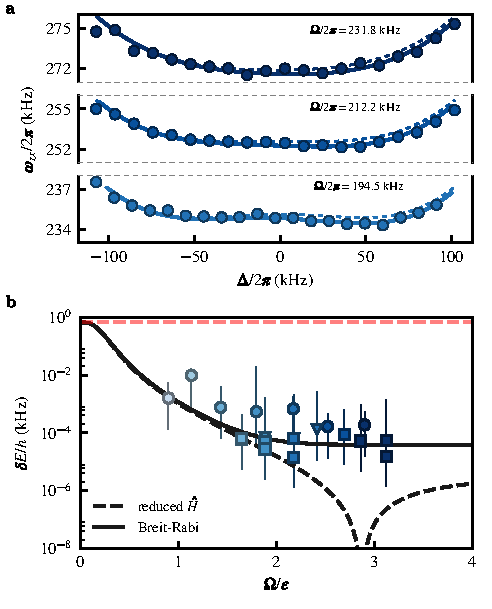
\includegraphics[]{Figures/Chapter6/fig2.pdf}
    \caption[The $\ket{z}\rightarrow\ket{x}$ transition as a function of $\Omega_{\rm RF}$]{(a) Transition frequency $\omega_{zx}/2\pi$ for three values of $\Omega/2\pi$.
    The dashed curves correspond to \refeq{eq:h}, while the solid curves use the Breit-Rabi expression.
    (b) The change in energy from our experimental detuning fluctuations as measured in the $m_F$ basis is $\delta \Delta/2\pi = \SI{0.67}{kHz}$ (red dashed line).
    Triangles correspond to $\xyz$ spectroscopy data, squares to side-of-peak $\pi$-pulse data, and circles to double-dressed data.
    The black dashed (solid) curve was calculated using \refeq{eq:h} (the Breit-Rabi expression).
    The shading of the data points corresponds to the Rabi frequencies in \reffig{fig:3}.}
    \label{fig:2}
\end{figure}



\section{System}

Our BECs had $N\approx\num{5e4}$ atoms, and were held in a crossed dipole trap with trapping frequencies $(f_x,\, f_y,\, f_z) = (42(3),\, 34(2),\, 133(3))$\,Hz~\footnote{All uncertainties herein represent the uncorrelated combination of statistical and systematic uncertainties.}.
The $B_0 \approx \SI{3.27}{mT}$ bias field lifted the ground state degeneracy, giving an $\omega_0/2\pi = \SI{22.9}{MHz}$ Larmor frequency, with a quadratic shift $\epsilon/2\pi=\SI{76.4}{kHz}$.
In our laboratory the ambient magnetic field fluctuations were dominated by contributions from line noise giving an rms uncertainty $\delta\Delta/2\pi = g_F \mu_{\rm B}\delta B/h=\SI{0.67(3)}{kHz}$.

We used adiabatic rapid passage (ARP) to transfer atoms initially prepared in any of the $\ket{m_F = 0,-1,1}$ states into the corresponding $\xyz$ states.  Beginning far from resonance ($\Delta(t=0)/2\pi \approx -\SI{450}{kHz}$) with all coupling fields off, we ramped on the RF dressing field in a two-step process. We first ramped from $\Omega=0$ to approximately half its final value in \SI{10}{ms}.
By increasing the magnetic field $B_0$, we then ramped $\Delta$ to zero in \SI{12}{ms} using a non-linear ramp adiabatic with respect to the relevant energy gaps.
After allowing $B_0$ to stabilize for \SI{30}{ms}, we ramped the RF dressing field to its final value $\Omega$ in \SI{10}{ms}, yielding the dynamically decoupled $\ket{y, x, z}$ states.

We measured the population in the $\xyz$ states, we adiabatically deloaded them back into the $m_F$ basis by ramping $B_0$ so that $\Delta$ approached its initial detuned value in \SI{2}{ms}, and then ramped off the dressing RF field in \SI{1}{ms}.
We obtained the spin-resolved momentum distribution using standard time-of-flight (TOF) imaging techniques, with a  Stern-Gerlach field to spatially separate the spin components during TOF.
The right panel of \reffig{fig:1}a shows such a TOF image for decomposition of $\ket z$ into the $m_F$ states in a typical TOF image.

We confirmed our control and measurement techniques spectroscopically measuring the energy differences between the $\xyz$ states with our prove field.
Figure~\ref{fig:1}b shows the dependence of the $\omega_{xy}/2\pi$, $\omega_{yz}/2\pi$, and $\omega_{zx}/2\pi$ on detuning for $\Omega/2\pi=\SI{194.5(1)}{kHz}$ derived from spectra such as in the side panel with coupling strength $\Omega_p/2\pi \approx \SI{1}{kHz}$ and $\Delta/2\pi \approx \SI{9}{kHz}$.

The dashed curves based on \refeq{eq:h} clearly depart from our measurements for the $zx$ transition.
This departure results from neglecting the weak dependence of the quadratic shift $\epsilon$ on bias field $B_0$.  In near-perfect agreement with experiment, the solid curves from the full Breit-Rabi expression account for this dependency.

\textit{Robustness.}
The $zx$ transition is remarkably robust against magnetic field variations, as commonly result from temporal and spatial magnetic field noise in laboratory environments  (Fig. \reffig{fig:2}a).
We focus on the $zx$ transition, which can be made virtually independent of magnetic field variations due to the similar curvature of $\omega_z(\Delta)$ and $\omega_x(\Delta)$ (see the middle panel of \reffig{fig:1}a).
We quantified the sensitivity of this transition to field variations with three methods corresponding to the different markers in \reffig{fig:2}b.
In each case we measured the energy shift from resonance as a function of detuning and then used a fourth order polynomial fit to extract the rms residuals $\delta \omega_{zx}$ due to the known detuning noise~\footnote{Our procedure also quantifies the small fluctuations that survive for spectra that are flat beyond second order, as in \refeq{eq:h}.}.
(1) Triangles denote data using full spectroscopical measurements similar to \reffig{fig:2}a.
(2) squares denote data in which a detuned $\pi$-pulse of the probe field transferred atoms from $\ket z$ to $\ket x$, a side-of-peak technique giving a signal first-order sensitive to changes in $\omega_{zx}$.
(3) circles describe data using an adiabatic technique described below.
The results are not consistent with the theory simple from \refeq{eq:h} (dashed) and instead require the Breit-Rabi expression (solid) to obtain full agreement~\footnote{The fluctuations can be even smaller for a given $\Omega$ if we allow for $\Delta \neq 0$ (see Supplemental Materials).}.

Even at our smallest coupling $\Omega/2\pi=\SI{69(1)}{kHz}$ the typical magnetic field noise was attenuated by two orders of magnitude, rendering it essentally undetectable.
Ideally, the radius of curvature of $\omega_{zx}(\Delta)$ changes sign at about $\Omega/2\pi = \SI{220}{kHz}$, leaving only a $\Delta^4$ contribution, however, in practice the small dependence of $\epsilon$ on $B$ prevents this perfect cancellation.
\begin{figure}[h]
    \centering
    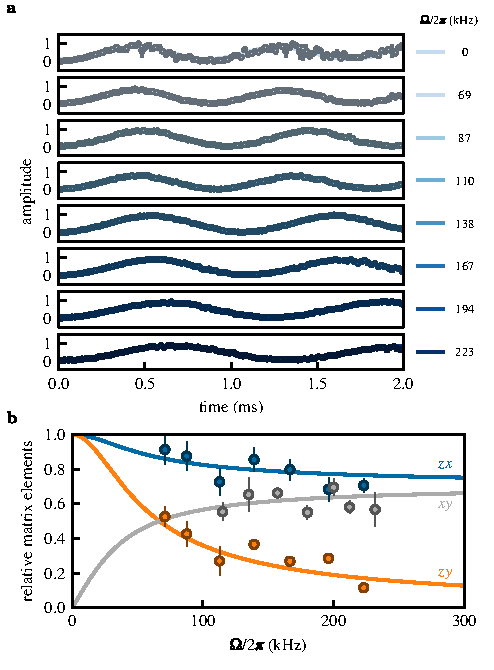
\includegraphics[]{Figures/Chapter6/fig3.pdf}
    \caption[Coherent driving of dressed state transitions]{(a) Rabi oscillations.
    Phase coherence is maintained throughout the oscillations in the dressed basis, while it is quickly lost in the $m_F$ basis.
    The marker size reflects the typical uncertainties on the dressed basis oscillations.
    (b) Transition matrix elements for $zx$ (blue) and $zy$ (orange) transitions decrease monotonically with increasing $\Omega$ for $\Delta=0$, while they increase for $xy$.
    }
    \label{fig:3}
\end{figure}

We explored the strength of the probe-driven transitions between these states by observing coherent Rabi oscillations (Fig. \reffig{fig:3}a) where our BEC was prepared in $\ket z$ and the probe field had strength $\Omega_p/2\pi\approx\SI{1}{kHz}$.
The top panel shows Rabi oscillations between $\ket{m_F=0}$ and $\ket{m_F=-1}$ states for reference, and the remaining panels show oscillations between $\ket{z}$ and $\ket{x}$.
The observed Rabi frequency between dressed states decreased with increasing $\Omega$ indicating a dependence of the $zx$ transition matrix elements on $\Omega$.
These matrix elements, as well as those for the $zy$ transition, decrease with increasing $\Omega$ for $\Delta=0$ as shown in \reffig{fig:3}b and Appendix~\ref{app:me}.
The coherence of the Rabi oscillations for longer times was limited by gradients in $\Omega$ that lead to phase separation of the dressed states, and therefore loss of contrast after a few tens of ms, but had no measurable effect on the coherence of the oscillations.
In comparison, the coherence of the Rabi oscillation between the $m_F$ states deteriorates after \SI{500}{\us}.
For these timescales, the loss of coherence was predominantly due to bias magnetic field temporal noise~\footnote{We cancelled gradient magnetic fields so that no phase separation of the bare states was observed for $>\SI{10}{sec}$.}.



\textit{Concatenated CDD.}
The driving field $\Omega$ coupled together the $\ket{m_F}$ states, giving us synthetic clock states $\xyz$ that were nearly insensitive to magnetic field fluctuations.
However, the spectrum of these states is first-order sensitive to fluctuations $\delta \Omega$ of the driving field.
Reference~\cite{cai_robust_2012} showed that an additional field coupling together these $\xyz$ states can produce doubly-dressed states that are insensitive to both $\delta \Omega$ and $\delta \Delta$: a process called concatenated CDD.
In our experiment, the probe field provided the concatenating coupling field.
Because $\Omega_p\ll\Omega$, we focus on a near-resonant two-level system formed by a single pair of dressed states, here $\ket{z}$ and $\ket{x}$, which we consider as pseudospins $\ket{\!\uparrow}$ and $\ket{\!\downarrow}$.
These are described by the effective two-level Hamiltonian
\begin{equation}
    \hat H_p = \frac{\hbar\Delta'}{2} \hat \sigma_3 + \hbar\Omega' \cos(\omega_p t) \hat \sigma_1,
    \label{eq:h2}
\end{equation}
with energy gap $\Delta' \approx \omega_{\downarrow, \uparrow}$ (shifted by off-resonant coupling to the $zy$ and $xy$ transitions) and coupling strength $\Omega' \propto \Omega_p$, as set by the matrix elements displayed in~\reffig{fig:3}b.
Here $\hat \sigma_{1,2,3}$ are the three Pauli operators.
\begin{figure}[h]
    \centering
    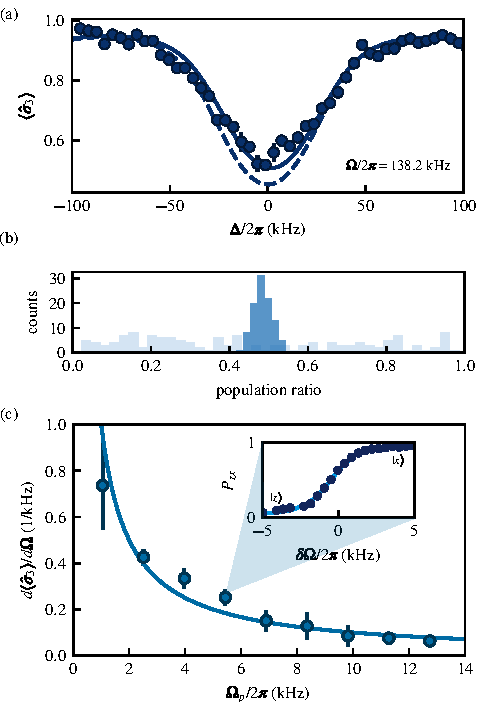
\includegraphics[]{Figures/Chapter6/fig4.pdf}
    \caption[Concatenated CCD]{(a) The fractional population imbalance of the $\downarrow\uparrow$ transition for $\Omega/2\pi=\SI{138.2(1)}{kHz}$ over detuning $\Delta$.
    The dashed curve is calculated using \refeq{eq:h} and the solid one using the full Breit-Rabi expression.
    (b) The fidelity of preparing a balanced superposition of $\ket{\!\downarrow}$ and $\ket{\!\uparrow}$ (dark blue) states compared to $\ket{m_F=0}$ and $\ket{m_F=-1}$ states (light blue).
    (c) The robustness of $\downarrow, \uparrow$ transition against fluctuations $\delta \Omega$ for different probe field coupling strengths.
    The points represent the slope of the fitted curves to the fractional population imbalance (inset).}
    \label{fig:4}
\end{figure}
A RWA of this Hamiltonian leads to the energy spectrum $E_{\uparrow,\downarrow} \approx \pm\Omega^\prime/2 + (\Delta^\prime)^2/2\Omega^\prime$, having again assumed the coupling $\Omega^\prime$ exceeds any fluctuations in $\Delta^\prime$.
Thus, the concatenated CDD field protects from the fluctuations $\delta\Delta\prime$ of the first dressing field in the same way that CDD provided protection from detuning noise $\delta \Delta$.


We produced doubly-dressed states by using the probe field near resonant with the $\downarrow, \uparrow$ transition and an ARP sequence.
We started in $\ket{\!\downarrow}$ at $\Delta=0$ and ramped on the probe field $\Omega_p$ a few ms before ramping $\Omega$ to its final value.
We chose  ARP parameters to create an equal superposition of $\ket{\!\downarrow}$ and $\ket{\!\uparrow}$ and quantified the sensitivity of this transition to large changes in the detuning in terms of the fractional population imbalance $\langle\hat\sigma_3\rangle = P_\downarrow(\Delta)-P_\uparrow(\Delta)$, shown in \reffig{fig:4}a for $\Omega/2\pi=\SI{138.2(1)}{kHz}$~\footnote{We chose the maximum value of $\Delta$ such that the population of \unexpanded{$\ket y$}, was negligible after deloading.}.
This signal is first-order sensitive to $\omega_{\downarrow, \uparrow}$, and provided our third measurement of sensitivity to detuning in \reffig{fig:2}b denoted by circles.

We compared the fidelity of preparing a superposition of the $\ket{\!\downarrow}$ and $\ket{\!\uparrow}$ states to adiabatically preparing a similar superposition of the the $\ket{m_F=0}$ and $\ket{m_F=-1}$ states, both with a probe field strength of  $\approx\SI{1}{kHz}$.
Figure~\ref{fig:4}b shows the rms deviation of the population imbalance measured over a few hundred repetitions of the experiment.
The rms deviation for the dressed basis is $0.024(1)$ and is and order of magnitude smaller than for the $m_F$ basis $0.29(1)$, where it practically impossible to prepare a balanced superposition for the parameters used here~\footnote{In \reffig{fig:4}b, the noise in the $m_F$ basis in not Gaussian distributed as is typical of line noise in these experiments.}.

Figure~\ref{fig:4}c shows the response of the $\downarrow, \uparrow$ transition to small changes $\delta\Omega$ for different values of $\Omega_p$.
We prepared an equal superposition of $\ket{\!\downarrow}$ and $\ket{\!\uparrow}$ following the same procedure as before for $\Omega/2\pi = \SI{138.2(1)}{kHz}$.
We then measured how the population imbalance changes for small variations of $\Omega$ --- the effective detuning in the `twice-rotated frame' --- for different probe amplitudes $\Omega_p$.
We defined a sensitivity parameter $d\langle\hat\sigma_3\rangle / d\Omega$, obtained from the linear regime of the population imbalance measurements (see inset in \reffig{fig:4}c).
The robustness of the doubly-dressed states against $\delta \Omega$ fluctuations increased with $\Omega_p$, thus verifying the concatenating effect of CDD in the $\xyz$ basis.

\textit{Conclusions.}
We realized a three-level system that is dynamically decoupled from low-frequency noise; measured now-allowed transitions between all three states; and demonstrated control techniques for creating arbitrary Hamiltonians.  These techniques add no heating or loss mechanisms, yet within the protected subspace retain the full complement of cold-atom coherent control tools such as optical lattices and Raman laser coupling, and permit new first-order transitions that are absent in the unprotected subspace.
These transitions enable experiments requiring a fully connected geometry as for engineering exotic states, e.g., in cold-atom topological insulators, and two-dimensional Rashba spin-orbit coupling in ultracold atomic systems~\cite{campbell_rashba_2016, juzeliunas_generalized_2010}.

The synthetic clock states form a decoherence-free subspace that can be used in quantum information tasks where conventional clock states might be absent, or incompatible with other technical requirements~\cite{bacon_universal_2000}.
Moreover, their energy differences are proportional to the amplitude of the dressing field, and hence tunable, so they can be brought to resonance with a separate quantum system.
The effective quantization axis can be arbitrarily rotated so that the two systems can be strongly coupled, pointing to applications in hybrid quantum systems~\cite{solano_chapter_2017,xiang_hybrid_2013}.
Introducing a second coupling field shields the system from fluctuations of the first, a process which can be concatenated as needed.
More broadly, synthetic clock states should prove generally useful in any situation where fluctuations of the coupling field can be made smaller than those of the environment.



\textit{Optimal response to noise}

The sensitivity of the $zx$ transition to detuning fluctuations can be optimized further by working at $\Delta \neq 0$ as shown in \reffig{fig:sopt}.
This behavior can only be captured by including the dependence of the quadratic shift on $\Delta$ as given by the Breit-Rabi expression.


For small values of $\Omega$ the optimum value of $\Delta$ corresponds to on of the concave features of the $zx$ transition energy that arise due to the asymmetry introduced by the quadratic shift.
As $\Omega$ gets larger, these features merge into a single one and the optimum value is $\Delta \approx 0$.
The deviation from $\Delta=0$ is due to an overall tilt of the transition energy coming from the dependence of the quadratic shift on $\Delta$.
At the optimum point $\Omega/\epsilon \approx 3$ the sensitivity of the synthetic clock transition is \SI{1.9e-07}{kHz}, c.f, the $\Rb87$ clock transition which scales as \SI{57.5}{kHz/mT^2} and gives \SI{5.8e-07}{kHz}.


\section{Locating field resonance}

We used an iterative procedure to measure and adjust the value of the detuning $\Delta$ to account for the weak response of the $\xyz$ states to detuning variations.
As most of our experiments were done at $\Delta=0$, we first obtained an estimate of $\Delta$ from the imbalance of $\ket 1$ and $\ket{-1}$ populations from the decomposition of $\ket z$ which should be zero for $\Delta=0$ (see \reffig{fig:s1}).
We then located the transition frequencies for at least two transitions (usually $zx$ and $zy$ as shown in \reffig{fig:s2}) using an ARP protocol as described in the main text and varying the frequency of the probe field.
These frequencies correspond to a unique pair of $\Omega$ and $\vert\Delta\vert$ values which can then be used to adjust the bias magnetic field $B_0$ so that $\Delta=0$.
However, there is an ambiguity as to the sign of $\Delta$ since the eigenstates are even functions of $\Delta$.


We selected a direction randomly and subsequently verified if $\Delta=0$ using another set of spectroscopic measurement.
We fixed the value of the probe field to be a few kHz above the transition frequency corresponding to $\Delta=0$ and used the same ARP sequence to transfer atoms from $\ket z$ to $\ket x$.
This procedure gave two resonant values for $\Delta$ were atom transfer takes place, and the value where $\Delta=0$ corresponded to their mean (see \reffig{fig:s2}).
Finally, we remeasured the $zx$ and $zy$ transition frequencies to validate that $\Delta=0$.
For higher values of $\Omega_R$, using the $zx$ transition becomes impractical
due to its insensitivity to detuning, and we followed the same procedure but using the $xy$ transition instead.




\section{System}
\subsection{The xyz basis}
State decomposition, matrix elements, detuning dependence of energy something about resonantly coupling them

\section{Experiments}
\subsection{State preparation and deloading}
\subsection{Finding zero detuning}


\section{Robustness}

\section{Concatenated CCD}




